\documentclass[journal,12pt,twocolumn]{IEEEtran}
\usepackage[compact]{titlesec}
\usepackage{setspace}
\usepackage{gensymb}
\singlespacing
\usepackage[cmex10]{amsmath}
\usepackage{amsthm}
\usepackage{mathrsfs}
\usepackage{txfonts}
\usepackage{stfloats}
\usepackage{bm}
\usepackage{cite}
\usepackage{cases}
\usepackage{subfig}
\usepackage{longtable}
\usepackage{multirow}
\usepackage{enumitem}
\usepackage{mathtools}
\usepackage{steinmetz}
\usepackage{tikz}
\usepackage{circuitikz}
\usepackage{verbatim}
\usepackage{tfrupee}
\usepackage[breaklinks=true]{hyperref}
\usepackage{tkz-euclide}

\usetikzlibrary{calc,math}
\usepackage{listings}
    \usepackage{color}                                            %%
    \usepackage{array}                                            %%
    \usepackage{longtable}                                        %%
    \usepackage{calc}                                             %%
    \usepackage{multirow}                                         %%
    \usepackage{hhline}                                           %%
    \usepackage{ifthen}                                           %%

    \usepackage{lscape}     
\usepackage{multicol}
\usepackage{chngcntr}

\DeclareMathOperator*{\Res}{Res}
\renewcommand\thesection{\arabic{section}}
\renewcommand\thesubsection{\thesection.\arabic{subsection}}
\renewcommand\thesubsubsection{\thesubsection.\arabic{subsubsection}}

\renewcommand\thesectiondis{\arabic{section}}
\renewcommand\thesubsectiondis{\thesectiondis.\arabic{subsection}}
\renewcommand\thesubsubsectiondis{\thesubsectiondis.\arabic{subsubsection}}

\hyphenation{op-tical net-works semi-conduc-tor}
\def\inputGnumericTable{}                                 %%

\lstset{
frame=single, 
breaklines=true,
columns=fullflexible
}

\begin{document}

\newtheorem{theorem}{Theorem}[section]
\newtheorem{problem}{Problem}
\newtheorem{proposition}{Proposition}[section]
\newtheorem{lemma}{Lemma}[section]
\newtheorem{corollary}[theorem]{Corollary}
\newtheorem{example}{Example}[section]
\newtheorem{definition}[problem]{Definition}
\newcommand{\BEQA}{\begin{eqnarray}}
\newcommand{\EEQA}{\end{eqnarray}}
\newcommand{\define}{\stackrel{\triangle}{=}}
\bibliographystyle{IEEEtran}

\providecommand{\mbf}{\mathbf}
\providecommand{\pr}[1]{\ensuremath{\Pr\left(#1\right)}}
\providecommand{\qfunc}[1]{\ensuremath{Q\left(#1\right)}}
\providecommand{\sbrak}[1]{\ensuremath{{}\left[#1\right]}}
\providecommand{\lsbrak}[1]{\ensuremath{{}\left[#1\right.}}
\providecommand{\rsbrak}[1]{\ensuremath{{}\left.#1\right]}}
\providecommand{\brak}[1]{\ensuremath{\left(#1\right)}}
\providecommand{\lbrak}[1]{\ensuremath{\left(#1\right.}}
\providecommand{\rbrak}[1]{\ensuremath{\left.#1\right)}}
\providecommand{\cbrak}[1]{\ensuremath{\left\{#1\right\}}}
\providecommand{\lcbrak}[1]{\ensuremath{\left\{#1\right.}}
\providecommand{\rcbrak}[1]{\ensuremath{\left.#1\right\}}}
\theoremstyle{remark}
\newtheorem{rem}{Remark}
\newcommand{\sgn}{\mathop{\mathrm{sgn}}}
\providecommand{\abs}[1]{\left\vert#1\right\vert}
\providecommand{\res}[1]{\Res\displaylimits_{#1}} 
\providecommand{\norm}[1]{\left\lVert#1\right\rVert}

\providecommand{\mtx}[1]{\mathbf{#1}}
\providecommand{\mean}[1]{E\left[ #1 \right]}
\providecommand{\fourier}{\overset{\mathcal{F}}{ \rightleftharpoons}}

\providecommand{\system}{\overset{\mathcal{H}}{ \longleftrightarrow}}
\newcommand{\solution}{\noindent \textbf{Solution: }}
\newcommand{\cosec}{\,\text{cosec}\,}
\providecommand{\dec}[2]{\ensuremath{\overset{#1}{\underset{#2}{\gtrless}}}}
\newcommand{\myvec}[1]{\ensuremath{\begin{pmatrix}#1\end{pmatrix}}}
\newcommand{\mydet}[1]{\ensuremath{\begin{vmatrix}#1\end{vmatrix}}}
\numberwithin{equation}{subsection}

\makeatletter
\@addtoreset{figure}{problem}
\makeatother
\let\StandardTheFigure\thefigure
\let\vec\mathbf

\renewcommand{\thefigure}{\theproblem}

\def\putbox#1#2#3{\makebox[0in][l]{\makebox[#1][l]{}\raisebox{\baselineskip}[0in][0in]{\raisebox{#2}[0in][0in]{#3}}}}
     \def\rightbox#1{\makebox[0in][r]{#1}}
     \def\centbox#1{\makebox[0in]{#1}}
     \def\topbox#1{\raisebox{-\baselineskip}[0in][0in]{#1}}
     \def\midbox#1{\raisebox{-0.5\baselineskip}[0in][0in]{#1}}
\vspace{3cm}
\title{Assignment-5}
\author{Vipul Kumar Malik}

\date{\today}

\maketitle
\newpage
\bigskip
\renewcommand{\thefigure}{\theenumi}
\renewcommand{\thetable}{\theenumi}

\begin{abstract}
This document explains the concept of finding the equation of circle using linear algebra.
\end{abstract}
Download all python codes from 
\begin{lstlisting}
https://github.com/vipulmalik8569/MT-EE5609
\end{lstlisting}
and latex-tikz codes from 
\begin{lstlisting}
https://github.com/vipulmalik8569/MT-EE5609
\end{lstlisting}
\section{\textbf{Problem}}
Find the equation of circle passing through the points
\begin{align}
    \vec{x_1}=\myvec{1\\1}, \vec{x_2}=\myvec{2\\-1}, \vec{x_3}=\myvec{8\\2}\label{eq:0}
\end{align}
\section{\textbf{Solution}}
Vector form of the equation of circle with radius $r$ and centered at $\vec{c}$ is :
\begin{align}
\vec{x}^T\vec{x}-2\vec{c}^T\vec{x}+\vec{c}^T\vec{c}-r^2=0\label{eq:1}
\end{align}
Where
\begin{align}
\vec{x}=\myvec{x\\y}, \vec{c}=\myvec{x_0\\y_0} 
\end{align}
For $\vec{x_1}$, $\vec{x_2}$ and $\vec{x_3}$ equation \eqref{eq:1} can be written as:
\begin{align}
\vec{x_1}^T\vec{x_1}-2\vec{c}^T\vec{x_1}+\vec{c}^T\vec{c}-r^2=0\\
\vec{x_2}^T\vec{x_2}-2\vec{c}^T\vec{x_2}+\vec{c}^T\vec{c}-r^2=0\\
\vec{x_3}^T\vec{x_3}-2\vec{c}^T\vec{x_3}+\vec{c}^T\vec{c}-r^2=0
\end{align}

In the matrix form this can be written as : 
\begin{align}
 \myvec{x_1&y_1&1&\vec{x_1}^T\vec{x_1}\\x_2&y_2&1&\vec{x_2}^T\vec{x_2}\\x_3&y_3&1&\vec{x_3}^T\vec{x_3}}\myvec{-2x_0\\-2y_0\\x_0^2+y_0^2-r^2\\1}&=\myvec{0\\0\\0\\0}\label{eq:2} 
\end{align}
By putting the values of $\vec{x_1},\vec{x_2}$ and $\vec{x_3}$ in \eqref{eq:2} we get :
\begin{align}
 \myvec{1&1&1&2\\2&-1&1&5\\8&2&1&68}\myvec{-2x_0\\-2y_0\\x_0^2+y_0^2-r^2\\1}&=\myvec{0\\0\\0\\0} \label{eq:3}
\end{align}
Using Gaussian Elimination method :
\begin{align}
\xleftrightarrow[R_3 \leftarrow 8R_1-R_3]{R_2 \leftarrow 2R_1-R_2}\myvec{1&1&1&2\\0&3&1&-1\\0&6&7&-52}\\
\xleftrightarrow{R_2 \leftarrow \frac{1}{3} R_2}\myvec{1&1&1&2\\[0.2cm]0&1&\frac{1}{3}&-\frac{1}{3}\\[0.2cm]0&6&7&-52}\\
\xleftrightarrow{R_3 \leftarrow 6R_2-R_3}\myvec{1&1&1&2\\[0.2cm]0&1&\frac{1}{3}&-\frac{1}{3}\\[0.2cm]0&0&-5&50}\label{eq:6}
\end{align}
Solving for $\vec{c}$ and $r$ using \eqref{eq:6} we get : 
\begin{align}
\myvec{-2x_0\\-2y_0\\x_0^2+y_0^2-r^2\\1}&=\myvec{-9\\-3\\10\\1}\\
\vec{c}=\myvec{x_0\\y_0}&=\myvec{\frac{9}{2}\\[0.1cm]\frac{3}{2}}\\
r^2&=12.5   
\end{align}
Putting these values in \eqref{eq:1}, the equation of circle is as follows : 
\begin{align}
\vec{x}^T\vec{x}-2\myvec{\frac{9}{2}\\[0.1cm]\frac{3}{2}}^T\vec{x}+\myvec{\frac{9}{2}\\[0.1cm]\frac{3}{2}}^T\myvec{\frac{9}{2}\\[0.1cm]\frac{3}{2}}-12.5&=0\label{eq:14}\\
x^2+y^2-9x-6y+10&=0\label{eq:15}
\end{align}
Plot of the circle given by equation \eqref{eq:15} is as follows :
\begin{figure}[h]
\centering
    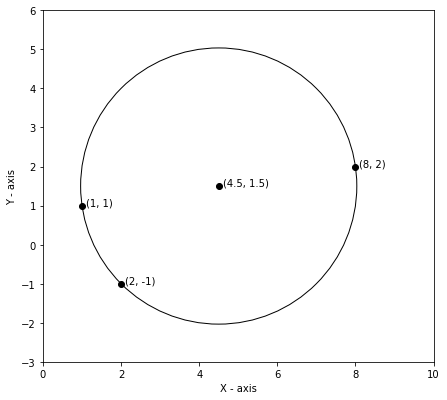
\includegraphics[width=\columnwidth]{circle2.png}
    \caption{A circle centered at $(4.5, 1.5)$ with radius $3.53$.}
    \label{circle}
\end{figure}
\end{document}

